\subsubsection{H-Brücke}
\label{subsubsec:H-Brücke}

Das Bindeglied zwischen Kraft (Motor) und Steuersignalen wird von der H-Brücke gebildet. Durch Laden-/Entladen der MOSFET-Gates wird die Spannung am Motor kommutiert.

\paragraph{Schaltungsaufbau}\mbox{}

Für den Aufbau und die Dimensionierung wurde das Referenzschema des Evaluationsboard verwendet, welches schon im Projekt 5 zum Einsatz gekommen ist (Trinamic UPS 10A70V). Das Schema ist im Anhang Kapitel \ref{Appendix:H_Bruecke_Referenzschema} zu finden. Die Dimensionierung der Shunts wurde in Kapitel \ref{subsubsec:Gate-Treiber} abgehandelt.

Der Schltungsaufbau ergibt sich durch den dreiphasigen Aufbau des BLDCs. Es werden so drei Stränge gebildet, woran jeweils eine Spule verbunden wird. Der Energiefluss führt dabei über einen Strommesswiderstand. Die Eingänge der H-Brücke werden zusätlich mit Stützkondensatoren bestückt, um eine saubere 48V-Netzspannung zu gewährleisten.

\begin{figure}[H]
	\centering
	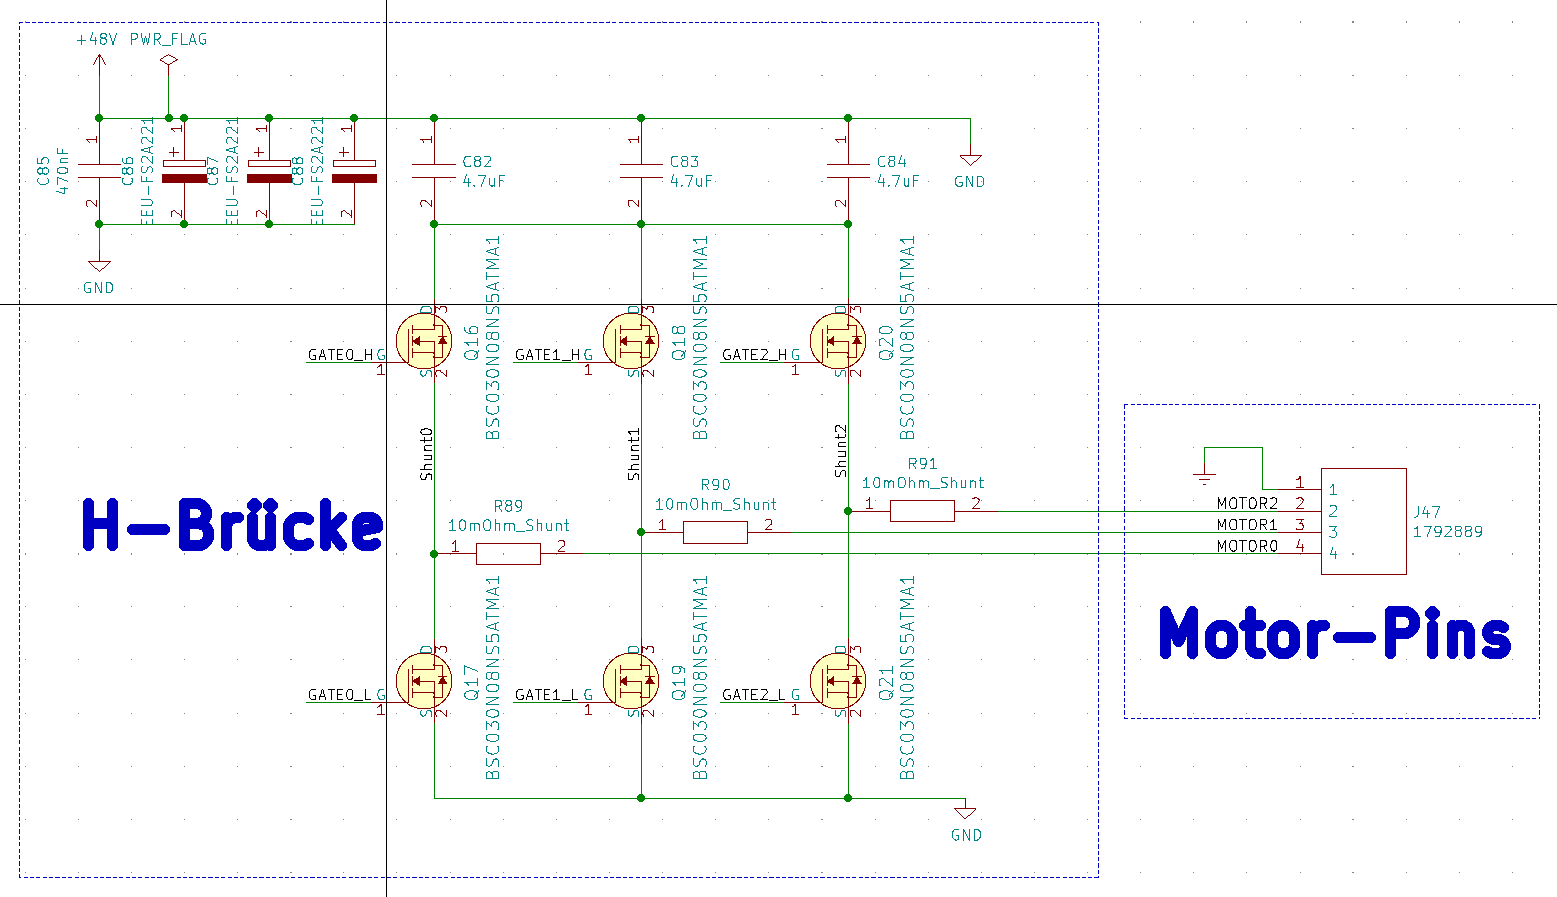
\includegraphics[width=\textwidth]{graphics/Schema_H_Bruecke_und_BLDC}
	\caption{H-Brücke.}
	\label{fig:Schema_H_Bruecke_und_BLDC}
\end{figure}

\paragraph{Funktionsbeschrieb der Schaltung}\mbox{}

Die Eingangsspannung der gesamte H-Brücke wird mit den Kondensatoren C85-C88 gestützt.
Bei C86-C88 handelt sich um Low-ESR Stützkondensatoren, jeweils ein Kondensator pro Phase.

Die Kondensatoren C82-C84 sind Kondensatoren, welche direkt zwischen Ein- und Ausgang eines H-Brücken-Strangs, nahe der MOSFETs platziert wurden.
Sie dienen auch zur Erhaltung der 48V-Versorgungsspannung.

Die MOSFETS Q16-Q21 bilden die eigentliche H-Brücke. Sie Schalten den Leistungsfluss gemäss den Gate-Ctrl-Signalen. Sie sinf für 100A Nennstrom und 100V Sperrspannung ausgelegt. Die Gate-Source-Spannung beträgt $\pm$20V.